\documentclass{standalone}
\usepackage{tikz}
\usepackage{ctex,siunitx}
\usepackage{tkz-euclide}
\usepackage{amsmath}
\usetikzlibrary{patterns, calc}
\usetikzlibrary {decorations.pathmorphing, decorations.pathreplacing, decorations.shapes,}
\begin{document}
\small
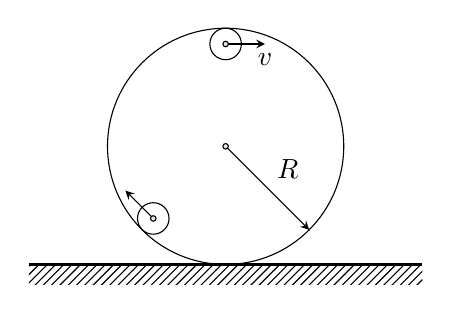
\begin{tikzpicture}[>=stealth,scale=1.0]
  \fill[pattern= north east lines](-2.5,-.25) rectangle (2.5,0); 
  \draw[thick](-2.5,0)--(2.5,0);
  \draw(0,1.5) circle (1.5);
  \draw[->](0,1.5)--+(-45:1.5)node[midway,above right]{$R$};
  \tkzDefPoints{0/2.8/R1, 0/1.5/R0, -.919/0.584/R2}
  \draw(R1) circle(.2);
  \draw(R2) circle(.2);
  \draw[->](R1)--+(.5,0)node[below]{$v$};
  \draw[->](R2)--+(135:.5);
  \tkzDrawPoints(R1,R0,R2)
\end{tikzpicture}
\end{document}